% Paquets généraux
\documentclass[a4paper,12pt,titlepage]{article}
\usepackage[T1]{fontenc}
\usepackage[utf8]{inputenc}
\usepackage[french]{babel}
\usepackage[gen]{eurosym}
%\usepackage[dvips]{graphicx}
\usepackage{fancyhdr}
\usepackage{pdfpages} 
\usepackage{multido}
\usepackage{hyperref}
%\usepackage{textcomp}
%\usepackage{aeguill}
\usepackage{schemabloc}
\usepackage[bitstream-charter]{mathdesign}
\usepackage{pstricks}
\usepackage{helvet}

\newcommand{\id}{54}
\newcommand{\nom}{Liaisons mécaniques}
\newcommand{\sequence}{04}
\newcommand{\num}{01}
\newcommand{\type}{TP}
\newcommand{\descrip}{Modélisation d'un solide. Comportement des liaisons mécaniques. Modéliser les mécanismes du laboratoire par un schéma cinématique, paramétré.}
\newcommand{\competences}{A3-C4: Analyse d'architecture et de comportement \\ &  Mod1-C1: Isolement d'un solide ou d'un système de solides \\ &  Mod2-C10-1: Modèle de solide indéformable \\ &  Mod2-C11: Modélisation géométrique et cinématique des mouvements entre solides indéformables \\ &  Mod2-C12: Modélisation cinématique des liaisons entre solides \\ &  Mod2-C15: Modélisation des actions mécaniques \\ &  Rés-C6: Utilisation d'un solveur ou d'un logiciel multi physique \\ &  Com1-C1: Différents descripteurs introduits dans le programme \\ &  Com2-C4: Outils de communication}
\newcommand{\nbcomp}{9}
\newcommand{\systemes}{Plateforme Stewart}
\newcommand{\systemessansaccent}{Plateforme Stewart}
\newcommand{\ilot}{2}
\newcommand{\ilotstr}{02}
\newcommand{\dossierilot}{\detokenize{Ilot_02 Plateforme Stewart}}
\newcommand{\imageun}{Plateforme}

\newcommand{\urlsysteme}{\href{https://www.costadoat.fr/systeme/57}{Ressources système}}
\newcommand{\matlabsimscape}{\href{https://github.com/Costadoat/Sciences-Ingenieur/raw/master/Systemes/Plateforme Stewart/Plateforme_Stewart_Simscape.zip}{Modèle Simscape}}
\newcommand{\solidworks}{\href{https://github.com/Costadoat/Sciences-Ingenieur/raw/master/Systemes/Plateforme Stewart/Plateforme_Stewart_Solidworks.zip}{Modèle Solidworks}}
\newcommand{\edrawings}{\href{https://github.com/Costadoat/Sciences-Ingenieur/raw/master/Systemes/Plateforme Stewart/Plateforme_Stewart.EASM}{Modèle eDrawings}}
\newcommand{\test}{Stewart_param1}
\newcommand{\testi}{Stewart_param2}
\newcommand{\testii}{Stewart_param3}
\newcommand{\testiii}{Stewart_param4}
\newcommand{\testiiii}{Stewart_euler}

\newcommand{\auteurun}{Renaud Costadoat}
\newcommand{\institute}{Lycée Dorian}


\usepackage{color}
\usepackage{xcolor}
\usepackage{colortbl}
\usepackage{helvet}
\renewcommand{\familydefault}{\sfdefault}
\usepackage{amsfonts}
\usepackage{amsmath}
%\usepackage{xspace}
\usepackage{varioref}
\usepackage{tabularx}
%\usepackage{floatflt}
\usepackage{graphics}
\usepackage{wrapfig}
\usepackage{textcomp}
\usepackage{tikz}
\usepackage{wrapfig}
\usepackage{gensymb}
\usepackage[european]{circuitikz}
\usetikzlibrary{babel}
\usepackage{ifthen}
\usepackage{cancel}
\usepackage{etoolbox}
\usepackage{multirow}
%\usepackage{boxedminipage}
\definecolor{gris25}{gray}{0.75}
\definecolor{bleu}{RGB}{18,33,98}
\definecolor{bleuf}{RGB}{42,94,171}
\definecolor{bleuc}{RGB}{231,239,247}
\definecolor{rougef}{RGB}{185,18,27}
\definecolor{rougec}{RGB}{255,188,204}%255,230,231
\definecolor{vertf}{RGB}{103,126,82}
\definecolor{vertc}{RGB}{220,255,191}
\definecolor{forestgreen}{rgb}{0.13,0.54,0.13}
\definecolor{blcr}{rgb}{0.59,0.69,0.84}
\definecolor{blfr}{rgb}{0.32,0.51,0.75}
\definecolor{orfr}{rgb}{0.90,0.42,0.15}
\definecolor{orcr}{rgb}{0.90,0.65,0.50}
\definecolor{orangef}{rgb}{0.659,0.269,0.072}
\definecolor{orange}{rgb}{0.58,0.35,0.063}
\definecolor{orangec}{rgb}{0.43,0.32,0.25}
\definecolor{rcorrect}{rgb}{0.6,0,0}
\definecolor{sequence}{rgb}{0.75,0.75,0.75}
\definecolor{competences}{rgb}{0.61,0.73,0.35}
\definecolor{grisf}{HTML}{222222}
\definecolor{grisc}{HTML}{636363}
\definecolor{normal}{HTML}{4087c4}
\definecolor{info}{HTML}{5bc0de}
\definecolor{success}{RGB}{92,184,92}
\definecolor{warning}{RGB}{240,173,78}
\definecolor{danger}{RGB}{217,83,79}
\hypersetup{                    % parametrage des hyperliens
    colorlinks=true,                % colorise les liens
    breaklinks=true,                % permet les retours à la ligne pour les liens trop longs
    urlcolor= blfr,                 % couleur des hyperliens
    linkcolor= orange,                % couleur des liens internes aux documents (index, figures, tableaux, equations,...)
    citecolor= forestgreen                % couleur des liens vers les references bibliographiques
    }

% Mise en page
\pagestyle{fancy}

\setlength{\hoffset}{-18pt}

\setlength{\oddsidemargin}{0pt} 	% Marge gauche sur pages impaire2s
\setlength{\evensidemargin}{0pt} 	% Marge gauche sur pages paires
\setlength{\marginparwidth}{00pt} 	% Largeur de note dans la marge
\setlength{\headwidth}{481pt} 	 	% Largeur de la zone de tête (17cm)
\setlength{\textwidth}{481pt} 	 	% Largeu\textbf{r de la zone de texte (17cm)
\setlength{\voffset}{-18pt} 		% Bon pour DOS
\setlength{\marginparsep}{7pt}	 	% Séparation de la marge
\setlength{\topmargin}{-30pt} 		% Pas de marge en haut
\setlength{\headheight}{55pt} 		% Haut de page
\setlength{\headsep}{20pt} 		% Entre le haut de page et le texte
\setlength{\footskip}{30pt} 		% Bas de\textbf{ page + séparation
\setlength{\textheight}{700pt} 		% Hauteur de l'icone zone de texte (25cm)
\setlength\fboxrule{1 pt}
\renewcommand{\baselinestretch}{1}
\setcounter{tocdepth}{1}
\newcommand{\cadre}[2]
{\fbox{
  \begin{minipage}{#1\linewidth}
   \begin{center}
    #2\\
   \end{center}
  \end{minipage}
 }
}

\newcommand{\reponse}[1][4]
{
\multido{}{#1}
{\begin{center}\makebox[0.9\linewidth]{}  \\
\begin{center}\makebox[0.9\linewidth]{\dotfill} \\ \end{center}
}}

\newcommand{\titre}[1]
{\begin{center}
\cadre{0.8}{\huge #1} 
\end{center}
}


% En tête et pied de page
\lhead{\nom}
\rhead{
\includegraphics[width=2cm]{../../img/logo}}
\lfoot{Renaud Costadoat}
\cfoot{Page \thepage}

\fancypagestyle{correction}{%
  \fancyhf{}
  \lhead{\colorbox{danger}{\begin{minipage}{0.65\paperwidth} \textcolor{white}{\textbf{Correction}} \end{minipage}} }
  \rhead{
\includegraphics[width=2cm]{../../img/logo}}
  \lfoot{Renaud Costadoat}
  \rfoot{\colorbox{danger}{\begin{minipage}{0.6\paperwidth} \begin{flushright}\textcolor{white}{\textbf{Correction}}\end{flushright} \end{minipage}} }}

\renewcommand{\footrulewidth}{0.4pt}

\usepackage{eso-pic}
\newcommand{\BackgroundPic}{%
\put(0,0){%
\parbox[b][\paperheight]{\paperwidth}{%
\vfill
\begin{center}
\hspace{0.5cm}\vspace{0.5cm}
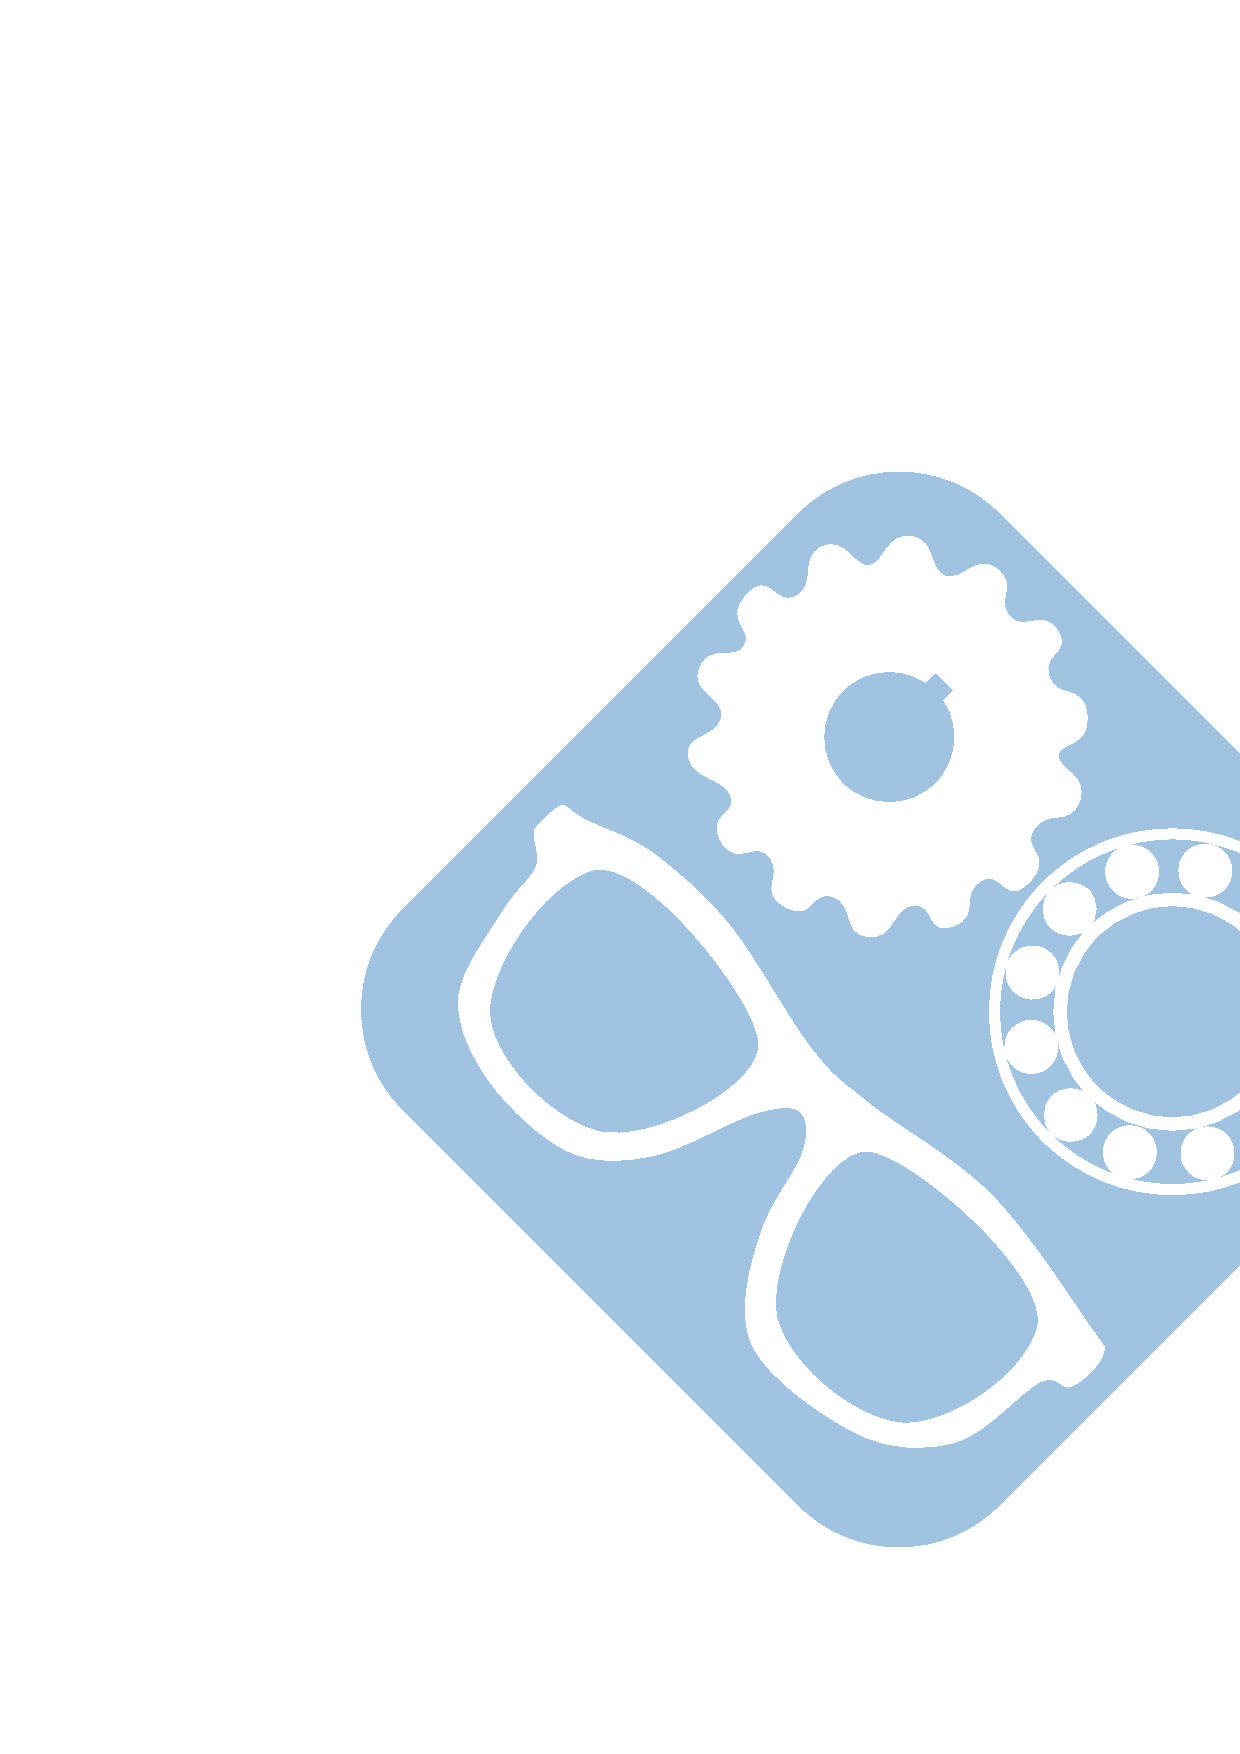
\includegraphics[width=\paperwidth,height=\paperheight,%
keepaspectratio]{../../img/fond3}%
\end{center}
\vfill
}}}

\newcommand{\BackgroundPicdeux}{%
\put(25,-30){%
\parbox[b][\paperheight]{\paperwidth}{%
\vfill
\begin{center}
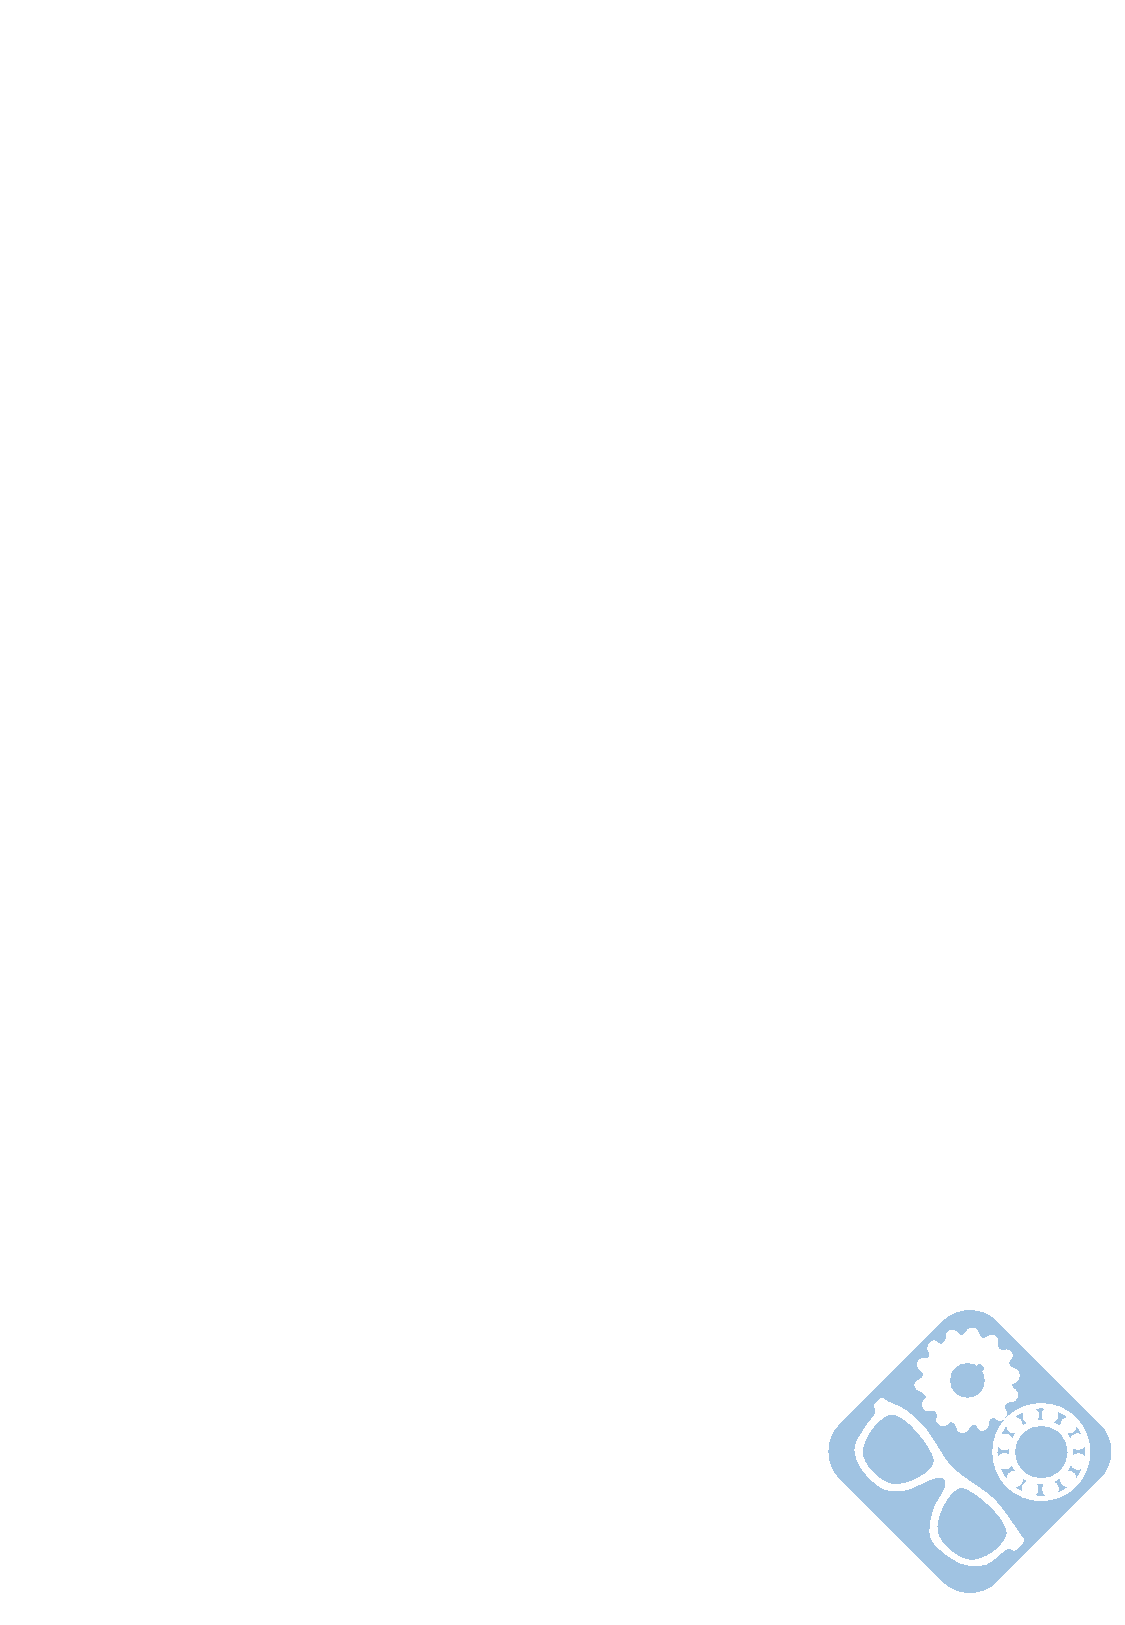
\includegraphics[width=\paperwidth,height=\paperheight,%
keepaspectratio]{../../img/fond4}%
\end{center}
\vfill
}}}

\begin{document}

\AddToShipoutPicture{\BackgroundPicdeux}

\pagestyle{fancy}

\section{Deux chariots avec Second Aller-Retour}

\begin{figure}[!h]
\begin{minipage}{0.55\linewidth}
Un chariot automatisé est un robot qui se déplace de façon autonome sans l'intervention humaine.

Ils sont le plus souvent utilisés dans des applications industrielles pour déplacer de manière autonome des marchandises dans une usine, un entrepôt, un atelier mais aussi des hôpitaux, musées, aéroports...
\end{minipage}
\hfill
\begin{minipage}{0.4\linewidth}
 \begin{center}
 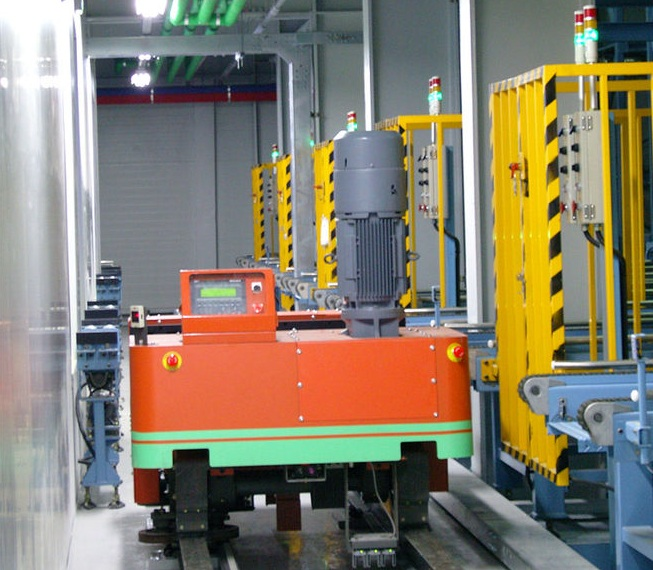
\includegraphics[width=0.6\linewidth]{img/chariot.jpg}
 \end{center}
 \caption{Chariot automatisé}
 \label{img1}
 \end{minipage}
\end{figure}

Un appui sur le bouton-poussoir \textbf{m} provoque la mise en marche de \textbf{D1} et de \textbf{D2} si le chariot \textbf{C1} est en \textbf{A1} et le chariot \textbf{C2} est en \textbf{A2}. Les deux chariots font un aller-retour. Le premier chariot qui revient à son point de départ effectue seul un second aller-retour. Si les deux chariots reviennent à leur point de départ au même instant, ils effectuent tous les deux un second aller-retour.

\begin{figure}[!h]
 \begin{center}
 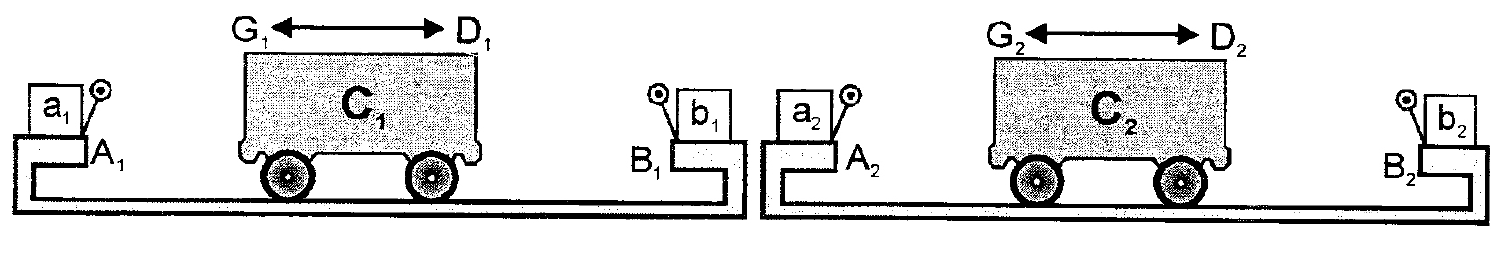
\includegraphics[width=0.8\linewidth]{img/Chariots_schema.png}
 \caption{Installation des chariots}
 \label{img2}
 \end{center}
\end{figure}

\paragraph{Question 1 :} Déterminer le grafcet point de vue partie opérative utilisant les spécificités technologiques de ce système.

\newpage

~\

\newpage

\section{Château d'eau}

\begin{figure}[!h]
\begin{minipage}{0.55\linewidth}
Un château d'eau est une construction destinée à entreposer l'eau, et placée en général sur un sommet géographique pour permettre de la distribuer sous pression.

L'entreposage de l'eau dans un réservoir joue un rôle de tampon entre le débit demandé par les abonnés et le débit fourni par la station de pompage. Il permet ainsi d'éviter de démarrer trop souvent les pompes et de les protéger. Une telle réserve permet également de faire face aux demandes exceptionnelles en cas d'incendie.

Un château d'eau est alimenté par trois pompes \textbf{P1}, \textbf{P2} et \textbf{P3} en fonction de l'état des trois détecteurs de niveau \textbf{h1}, \textbf{h2} et \textbf{h3}. Un détecteur de niveau est à l'état 1 s'il est noyé.
\end{minipage}
\hfill
\begin{minipage}{0.4\linewidth}
 \begin{center}
 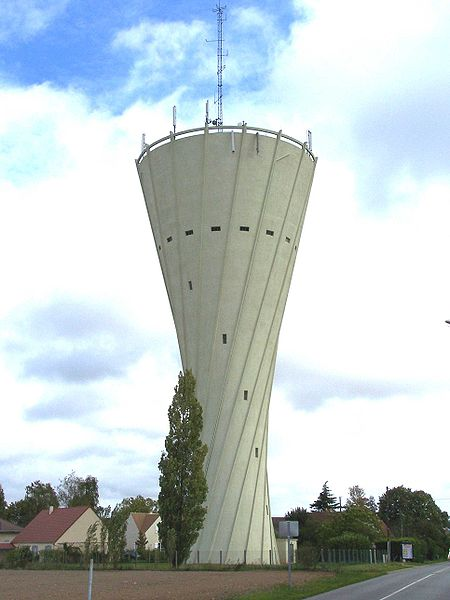
\includegraphics[width=0.7\linewidth]{img/chateau-eau.jpg}
 \end{center}
 \caption{Château d'eau}
 \label{img3}
 \end{minipage}
\end{figure}

\begin{figure}[!h]
 \begin{minipage}{0.4\linewidth}
  \begin{center}
   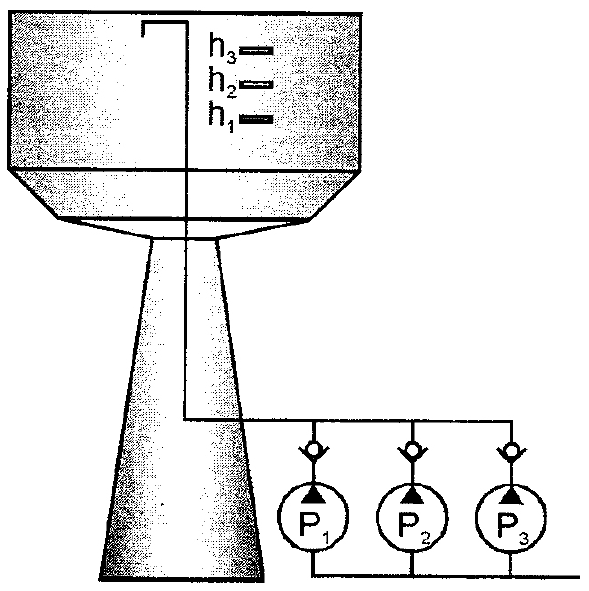
\includegraphics[width=0.9\linewidth]{img/Chateau_schema.png}
   \caption{Château d'eau}
   \label{img4}
  \end{center}
 \end{minipage}
 \hfill
 \begin{minipage}{0.55\linewidth}
  \textbf{Cahier des charges n°1 :}

  Un interrupteur \textbf{m} permet de mettre en fonctionnement l'installation.

  La pompe \textbf{Pi} est en fonctionnement si l'interrupteur \textbf{m} est actionné et si le détecteur de niveau \textbf{hi} n'est pas noyé.

 \paragraph{Question 1 :} Établir le grafcet point de vue partie opérative du système.
  
 \end{minipage}
\end{figure}

\textbf{Cahier des charges n°2 :}

Le fonctionnement, décrit précédemment, fait apparaître une utilisation excessive de la pompe \textbf{P3} ce qui provoque son échauffement et diminue sa durée de vie. Pour éviter ces inconvénients, on décide d'effectuer une permutation circulaire de l'utilisation des pompes, à chaque front montant de \textbf{h3} ou de l'interrupteur \textbf{m}.

\paragraph{Question 2 :} Établir le grafcet point de vue partie opérative du système.

\newpage

~\

\newpage

\section{Tableau de classe motorisé}

Dans une salle de classe on désire installer un tableau double à commande électrique.

\begin{figure}[!h]
\begin{minipage}{0.55\linewidth}
Le dispositif est le suivant :
\begin{itemize}
 \item Un moto-réducteur \textbf{MR} commande une vis sans fin actionnant le tambour sur lequel un câble s'enroule.
 \item Le câble est lié au tableau avant \textbf{av} et au tableau arrière \textbf{ar}.
 \item Le moteur est commandé par un contacteur marche-avant \textbf{CH} pour le sens \textbf{H} et un contacteur marche-arrière \textbf{CB} pour le sens \textbf{B}.
 \item Le bouton \textbf{m} permet la montée du tableau avant, tant qu'il est appuyé. Si on relâche \textbf{m} le tableau s'arrête.
 \item Le bouton \textbf{d} assure la descente du tableau avant, tant qu'il est appuyé. Si on relâche \textbf{d} le tableau s'arrête.
\end{itemize}
\end{minipage}
\hfill
\begin{minipage}{0.4\linewidth}
 \begin{center}
 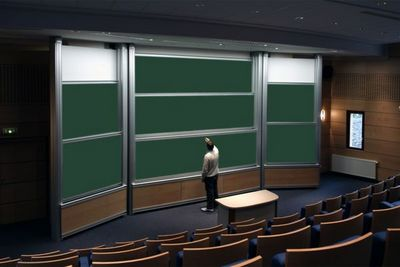
\includegraphics[width=1\linewidth]{img/Tableau.jpg}
 \end{center}
 \caption{Tableau d'amphithéâtre}
 \label{img5}
 \end{minipage}
\end{figure}

Fonctionnement
\begin{itemize}
 \item Le tableau avant se déplace vers le haut, lorsque le moteur tourne dans le sens \textbf{H}.
 \item Le tableau avant se déplace vers le bas, lorsque le moteur tourne dans le sens \textbf{B}.
\end{itemize} 

Condition supplémentaire :
\begin{itemize}
 \item L'action simultanée sur \textbf{m} et \textbf{d} provoque l'arrêt du moteur qui ne se remet en marche que lorsque l'un des deux boutons est libéré et dans le sens prescrit par celui qui reste appuyé.
\end{itemize} 

\paragraph{Question 1 :} Réaliser un schéma indiquant la position des tableau, des effecteurs et des capteurs.

\paragraph{Question 2 :} Donner la table de vérité permettant de décrire le fonctionnement du système.

\paragraph{Question 3 :} En déduire les équations logiques, puis les schémas à contacts, et enfin les logigrammes permettant de décrire le fonctionnement du système.

\paragraph{Question 4 :} Donner le schéma de câblage :
\begin{itemize}
 \item du circuit de commande (alimentation électrique continue 5V),
 \item du circuit de puissance (alimentation électrique triphasée 220V).
\end{itemize}

Prise en compte des butées :
Pour éviter de détériorer les butées des tableaux ou de faire surchauffer le moteur, on rajoute des détecteurs 
de fin de course position haute \textbf{phav} pour le tableau avant et position haute pour le tableau arrière \textbf{phar}.

\paragraph{Question 5 :} En déduire les nouvelles équations logiques et enfin les logigrammes permettant de décrire le 
fonctionnement du système.

\newpage

~\

\newpage

\section{Escalator avec contrôle d'accès}

\begin{figure}[!h]
\begin{minipage}{0.55\linewidth}
Dans une ambassade, afin d'assurer la sécurité et de contrôler le nombre de personnes qui rentrent, on les oblige à emprunter un escalier mécanique menant à l'étage où se situent les bureaux.

Dans cet escalier, une seule personne à la fois peut prendre place. Pour monter dans l'escalier, il faut que la personne franchisse un portillon à tourniquet semblable à ceux que l'on rencontre dans le métro.
\end{minipage}
\hfill
\begin{minipage}{0.4\linewidth}
 \begin{center}
 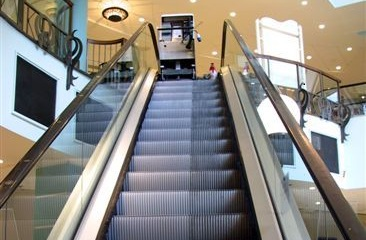
\includegraphics[width=0.8\linewidth]{img/escalator.jpg}
 \end{center}
 \caption{Tableau d'amphithéâtre}
 \label{img6}
 \end{minipage}
\end{figure}

Le fonctionnement de cette machine est décrit ci-dessous :
\begin{enumerate}
 \item Lorsqu'une personne franchit le portillon, elle pose le pied sur un tapis sensible \textbf{tb} placé en bas de l'escalier, aussitôt, l'escalier se met en marche \textbf{M},
 \item Dès que la personne pose un pied sur l'escalier, tout en gardant l'autre sur le tapis sensible, son poids est détecté par un capteur \textbf{c} qui indique la présence de la personne dans l'escalier. Dès que ce capteur \textbf{c} est activé, un verrou \textbf{V} réalisé avec un vérin à simple effet est commandé pour bloquer le portillon, et l'escalier continue de marcher \textbf{M},
 \item Tout le temps que la personne va être dans l'escalier, le verrou \textbf{V} sera activé, et l'escalier sera en marche \textbf{M},
 \item Dès que la personne arrive en haut de l'escalier, elle pose le pied sur un autre tapis sensible \textbf{th}, mais il faut qu'elle quitte l'escalier \textbf{c}, pour que celui-ci s'arrête de marcher, par contre le verrou \textbf{V} reste actif,
 \item Enfin, lorsque la personne quitte le tapis sensible du haut \textbf{th}, le verrou \textbf{V} est désactivé,
 \item Un tel cycle garantit qu'une seule personne à la fois puisse prendre l'escalier. Mais si par hasard, il arrivait un cas indésirable, alors toute action devrait être désactivée, afin d'assurer la sécurité et de réparer la panne.
\end{enumerate}

\paragraph{Question 1 :} Donner la table de vérité permettant de décrire le fonctionnement du système.

\paragraph{Question 2 :} En déduire les équations logiques simplifiées, puis les schémas à contacts, et enfin les  logigrammes permettant de décrire le fonctionnement du système.

\newpage

~\

\newpage

\section{Système de freinage de l'A318}


Il existe deux modes de commande du système de freinage :
\begin{itemize}
\begin{minipage}{0.6\linewidth}
 \item \textbf{le mode normal} (Normal Braking) contrôlé par un ordinateur dénommé \textbf{BSCU} (Braking/Steering Control Unit). Le \textbf{BSCU} contrôle les servovalves (une par roue) qui alimentent les pistons presseurs du système de freinage. La pression hydraulique est fournie par le groupe hydraulique principal.
\end{minipage}
\hfill
\begin{minipage}{0.38\linewidth}
 \centering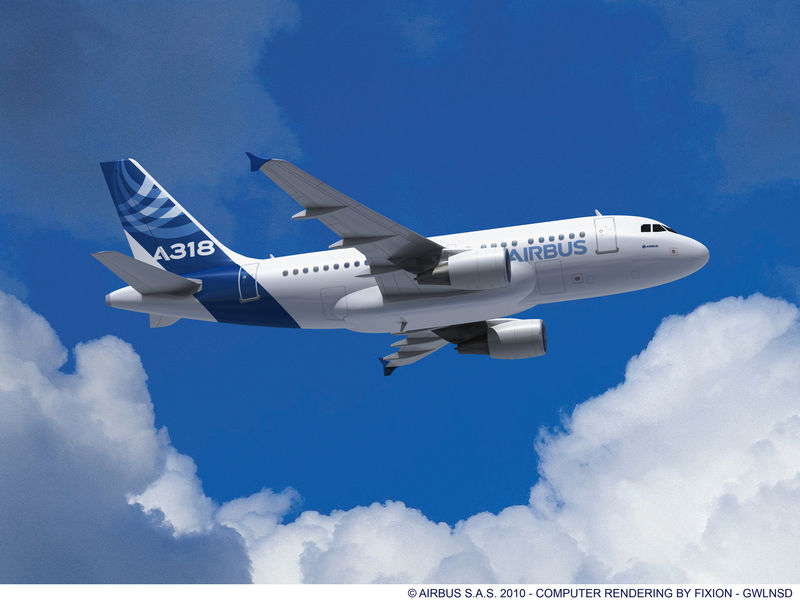
\includegraphics[width=0.7\linewidth]{img/A318.jpg}
 \vspace{0.5cm}
\end{minipage}
 \item \textbf{le mode alternatif} (Alternate braking) contrôlé par un ordinateur dénommé \textbf{ABCU} (Alternate Braking Control Unit). Ce mode prend automatiquement la relève du mode normal s'il y a dysfonctionnement de ce dernier ou si le contrôle anti-dérapage (Anti-Skid) de l'avion est supprimé. En mode alternatif, la pression hydraulique est fournie par un groupe hydraulique secondaire.
\end{itemize}

\begin{figure}[!h]
\begin{minipage}{0.38\linewidth}
 \begin{center}
 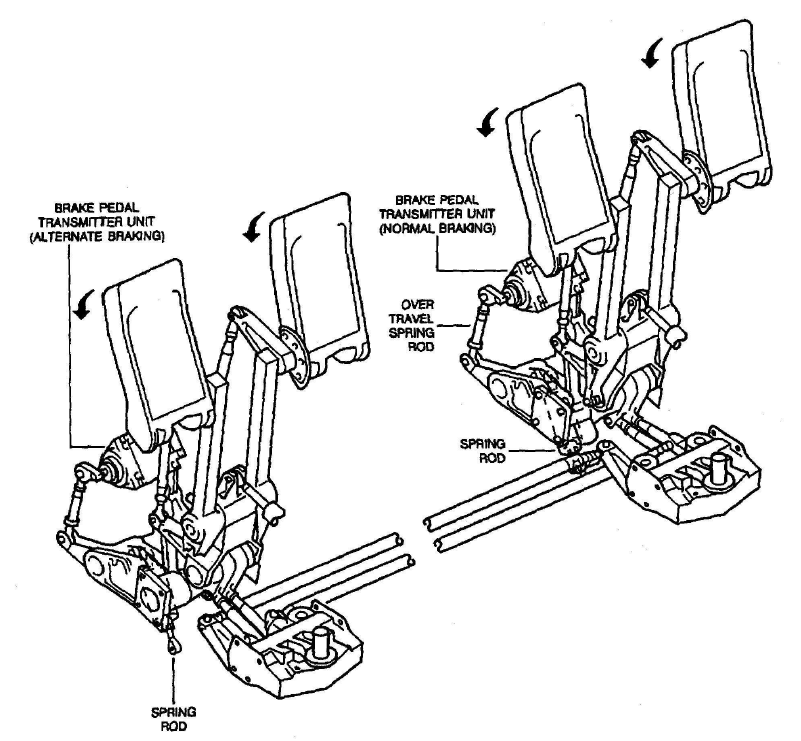
\includegraphics[width=0.7\linewidth]{img/Frein.png}
 \caption{Pédales de frein}
 \label{img7}
 \vspace{0.5cm}
  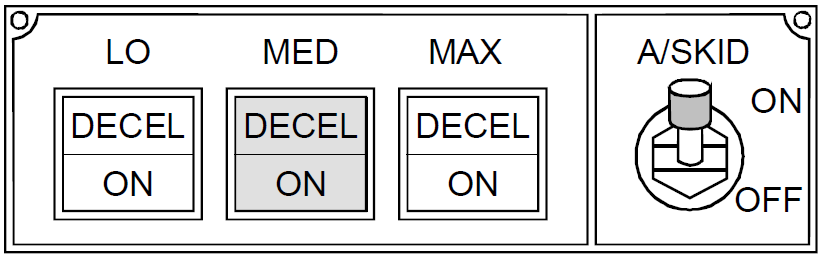
\includegraphics[width=0.5\linewidth]{img/Frein2.png}
 \caption{Tableau de bord}
 \label{img8}
  \end{center}
\end{minipage}\hfill
\begin{minipage}{0.6\linewidth}
En mode normal, il est possible de commander le freinage de deux façons différentes :
\begin{itemize}
 \item soit manuellement par appui sur les pédales de frein, figure \ref{img7}. La pédale gauche agit sur les roues du train gauche, l'appui sur celle de droite sur le train droit. Les unités de transmission (Brake Pedal Transmitter Unit) situés sous les pédales émettent des signaux électriques vers le \textbf{BSCU} ou vers l'\textbf{ABCU} proportionnels à la course des pédales de frein.
 \item soit automatiquement suivant trois modes de décélération : \textbf{LO}, \textbf{MED}, \textbf{MAX}. La sélection se fait à partir de trois boutons situés sur le tableau de bord, figure \ref{8}. Le mode manuel est rétabli si le pilote, en appuyant sur les pédales de frein, génère une consigne de décélération $ap$ supérieure à la consigne de décélération $a_c$ du mode automatique sélectionné.
\end{itemize} 
\end{minipage}
\end{figure}

Les modes \textbf{LO} et \textbf{MED} sont utilisés lors de l'atterrissage. Ils correspondent respectivement à une décélération de l'avion de $1,7m.s^{-2}$ et de $3m.s^{-2}$. Le mode \textbf{MAX} est exclusivement sélectionné lors du décollage, en cas d'interruption de ce dernier. Il correspond à une décélération théorique de $10m.s^{-2}$ supérieure à la décélération maximale de l'avion.

En mode normal (manuel ou automatique), le \textbf{BSCU} contrôle l'anti-dérapage (Anti Skid) de chaque roue tant que la vitesse de l'avion est supérieure à $5m.s^{-1}$.

En mode alternatif, seule la commande manuelle est disponible avec ou sans anti-dérapage.

Le grafcet de la figure \ref{img10} représente de façon très simplifiée la commande du système de freinage.

\paragraph{Question 1 :} La réceptivité (1) du grafcet \textbf{G1} est $(LO+MED+MAX).\left[a_p<a_c]\right[$. Donner l'expression de la réceptivité (2) sachant qu'elle est le complément de la réceptivité (1).

\paragraph{Question 2 :} Préciser quelles sont les étapes actives en situation initiale.

\paragraph{Question 3 :} On est en situation initiale. Les conditions suivantes sont réunies :
\begin{itemize}
 \item le freinage est sollicité,
 \item le mode MED est sélectionné,
 \item il n'y a pas de défaillance,
 \item le pilote n'agit pas sur les pédales de frein,
 \item l'A/Skid est enclenché.
\end{itemize}

Décrire la succession des situations fugaces atteintes par le grafcet de commande avant d'arriver sur une situation stable.

\paragraph{Question 4 :} On est dans la situation stable précédente et le pilote retire l'anti-skid. Décrire comme précédemment les évolutions au sein du grafcet.

\paragraph{Question 5 :} Expliquer et justifier la représentation suivante pour la détermination de la consigne de
décélération.

\begin{figure}[!h]
 \begin{center}
 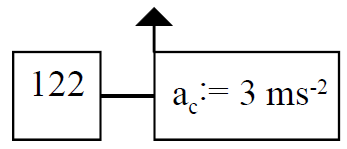
\includegraphics[width=0.3\linewidth]{img/Frein3.png}
 \caption{Etape 122}
 \label{img9}
 \end{center}
\end{figure}

\newpage

\begin{figure}[!h]
 \begin{center}
 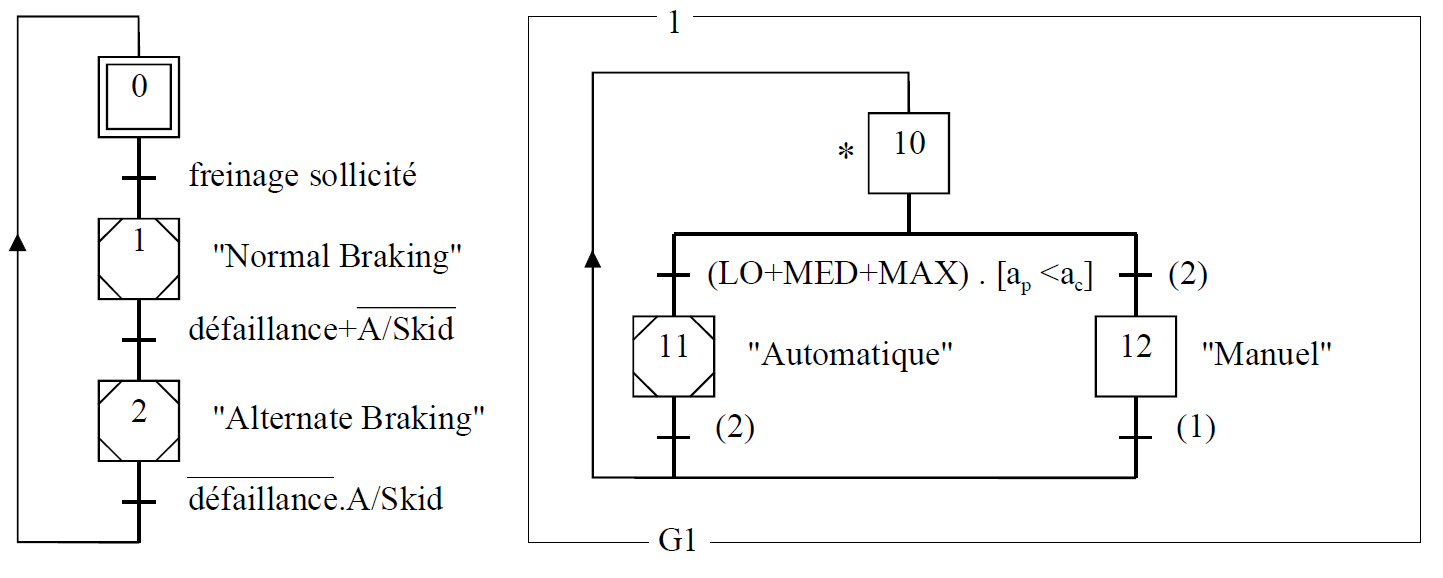
\includegraphics[width=1\linewidth]{img/Frein4.png}
 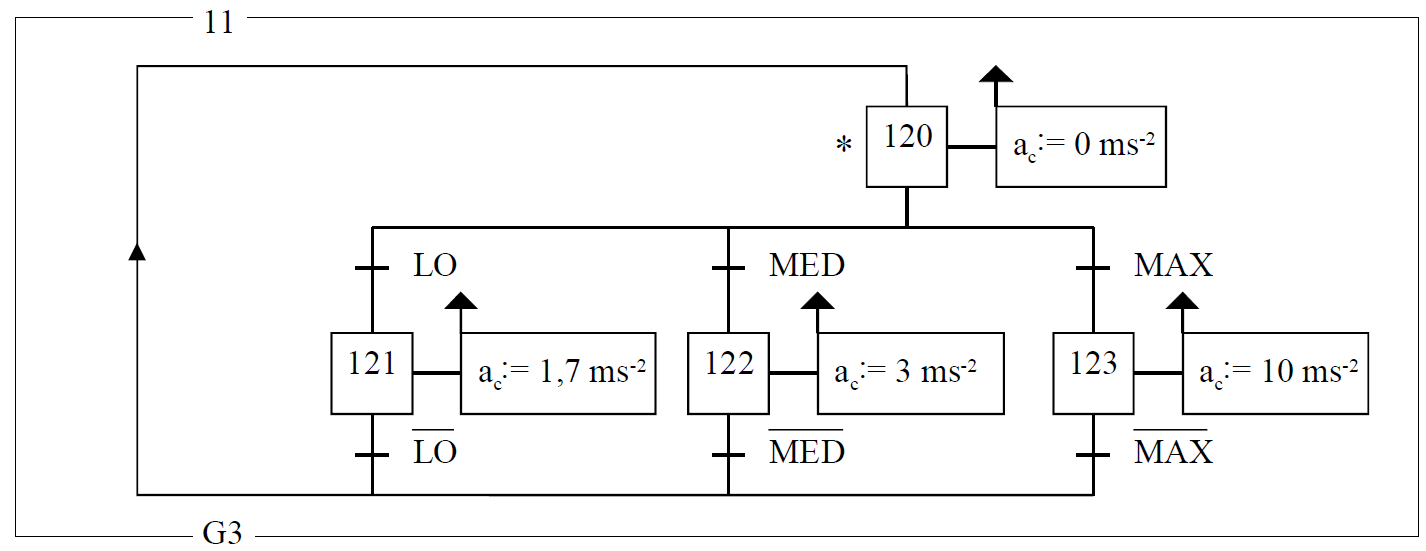
\includegraphics[width=1\linewidth]{img/Frein5.png}
 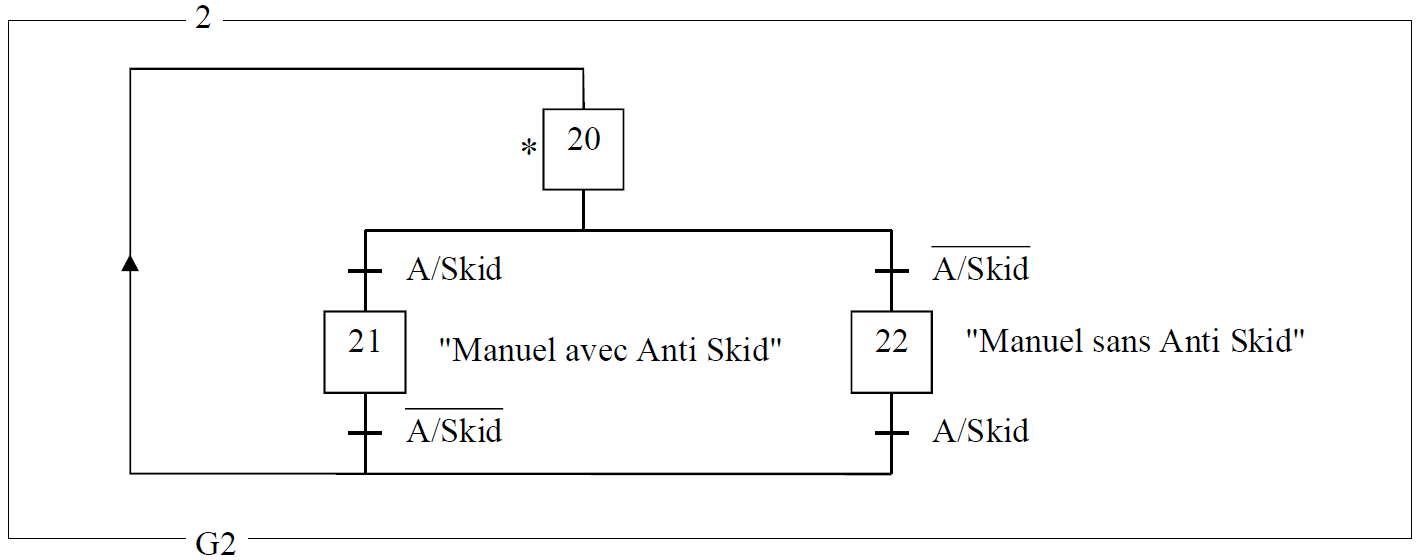
\includegraphics[width=1\linewidth]{img/Frein6.png}
  \caption{Grafcets}
 \label{img10}
 \end{center}
\end{figure}

\newpage

~\

\newpage

\end{document}